\chapter{Brudgrænsetilstand}

I dette afsnit undersøges tilbygningens brudgrænsetilstand. Først beregnes reaktionerne ud fra Figur \ref{fig:alle} og dernæst laves snitkræfter. Slutteligt undersøges spændingstilstanden, og udfra ståltypens flydespændingen kan det vurderes, om konstruktionen kan holde eller vil bryde sammen.   

\section{Reaktioner}
Reaktionerne i de tre understøtninger beregnes ved at opdele konstruktionen. Systemet opdeles i det midterste charnierled i henholdvis en venstre- og højre del, som ses på Figur \ref{fig:opdelingv} og \ref{fig:opdelingh}. I skæringen mellem de to dele, vil der være snitkræfter, men ikke momentkræfter, da momentet i charnierledet er nul. Dermed optræder der kun normalkraften, N, og forskydningskraften, V. Det er derfor muligt, at betragte højre del som et isoleret del af konstruktionen med fast, simpel understøtning i punkt E.

\begin{figure}[H]
	\centering
	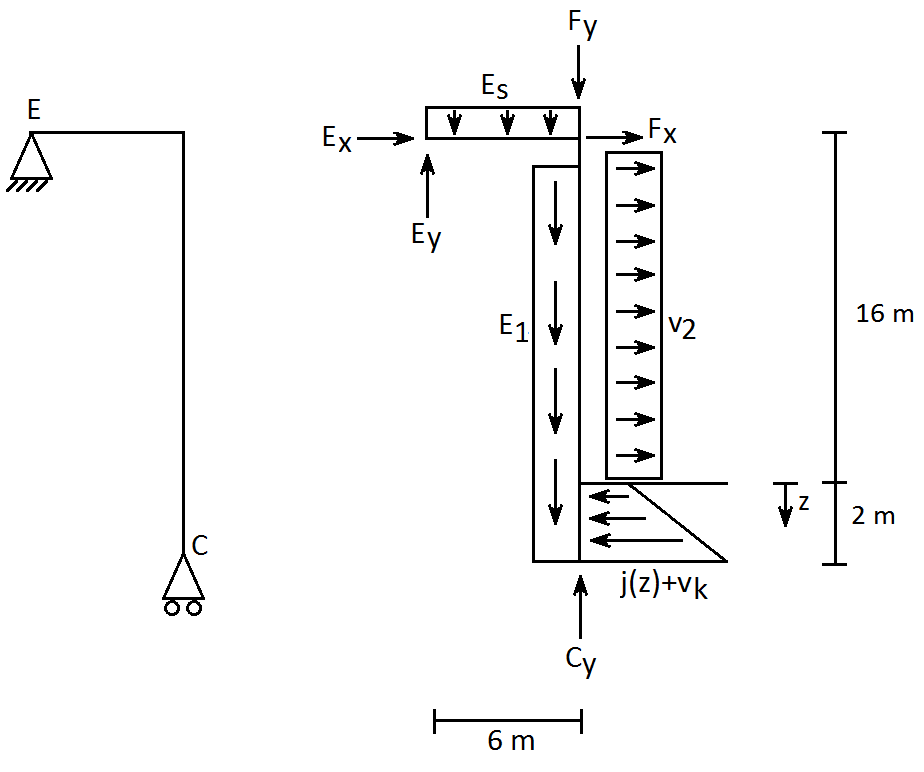
\includegraphics[width=0.7\textwidth]{billeder/hojre.png}
	\caption{Højre side af systemet, samt fritlegemediagram}
	\label{fig:opdelingh}
\end{figure}

\begin{figure}[H]
	\centering
	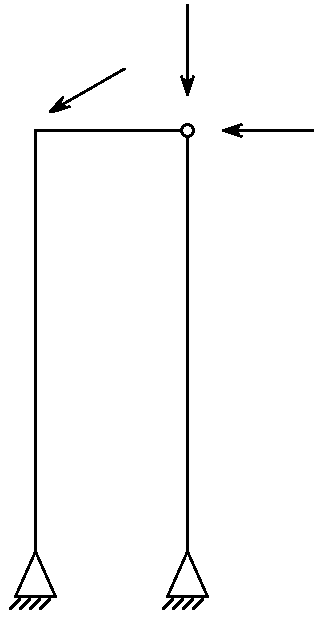
\includegraphics[width=0.7\textwidth]{billeder/venstre.png}
	\caption{Venstre side af systemet, samt fritlegemediagram}
	\label{fig:opdelingv}
\end{figure}

Reaktionerne i punkt E kan sættes som punktlaster på den venstre side af systemet, som ses på Figur \ref{fig:opdelingv}. Reaktionerne på højre del af systemet beregnes først.
\newline
\newline
Først bestemmes den vandrette reaktion i charnier ledet, $E_x$ gennem vandret ligevægt: 
\begin{center}
	$\rightarrow+:0 = F_x + E_x - J(2m) - V_k \cdot 2m - V_2 \cdot 16m$
	\newline
	$E_x = -1,\!45 kN$
\end{center}

$C_y$ bestemmes gennem moment ligevægt om punkt E: 
\begin{center}
	$\AR{}:0 = -F_y \cdot 6m - E_1 \cdot 18m \cdot 6m + C_y \cdot 6m - J(2m) \cdot 17,\!33m - V_k \cdot 2m \cdot 17m - E_s \cdot 6m \cdot 3m - V_2 \cdot 16m \cdot 8m$
	\newline
	$C_y = 779,\!83 kN$
\end{center}

Til sidst bestemmes den lodrette reaktion i charnier ledet, $E_y$ gennem lodret ligevægt: 
\begin{center}
	$\uparrow+: 0 = F_y - E_1 \cdot 18m - E_s \cdot 6m + C_y + E_y$
	\newline	
	$E_y = -164,\!89 kN$
\end{center}

Reaktionerne $E_y$ og $E_x$ påsættes som belastninger i punkt E på det venstre system, så de virker som vist på Figur \ref{fig:opdelingv}. Reaktionerne i det venstre system kan hermed bestemmes.
\newline
\newline
Først tages der moment om A, for at beregne $B_y$:
\begin{center}
	$A\hookrightarrow+: 0 = B_y \cdot 6m + E_y \cdot 6m + E_x \cdot 18m - E_2 \cdot 18m \cdot 6m - E_s \cdot 6m \cdot 3m + D_x \cdot 18m - V_1 \cdot 16m \cdot (8m + 2m) - J(2m) \cdot (2m \cdot \frac{1}{3}) - V_k \cdot 2m \cdot 1m$
	\newline 
	$B_y = 127,\!92 kN$
\end{center}

Nu laves lodret ligevægt for at bestemme $A_y$:
\begin{center}
	$\uparrow+: 0 = A_y + B_y - E_y - E_2 \cdot 18m - E_1 \cdot 18m - F_y - E_s \cdot 6 m$
	\newline
	$A_y = 547,\!96 kN$
\end{center}

For at gøre det muligt at isolere en af de vandrette reaktioner laves der et snit i charnieret. Derefter betragtes den nedre del, og der tages moment omkring charnieret i punkt E, for at bestemme $B_x$:
\begin{center}
	$\hookrightarrow+: 0 = B_x \cdot 18m$
	\newline
	$B_x = 0 kN$
\end{center}

Slutteligt laves vandret ligevægt for at bestemme $A_x$:
\begin{center}
	$\rightarrow+: 0 = A_x - E_x + B_x + J(2m) + V_k \cdot 2m + V_1 \cdot 16 m - D_x$
	\newline
	$A_x = -133,\!31 kN$
\end{center} 

\section{Snitkræfter}
Snitkræfterne for stålrammen til tilbygningen til Strøybergs Palæs kan nu beregnes. Her laves der syv snit, som er illustreret på Figur \ref{fig:snitbrud}. Disse resultater vil bruges til at undersøge, om konstruktionen har en tilstrækkelig bæreevne, eller om den vil bryde sammen. 

\begin{figure}[H]
	\centering
	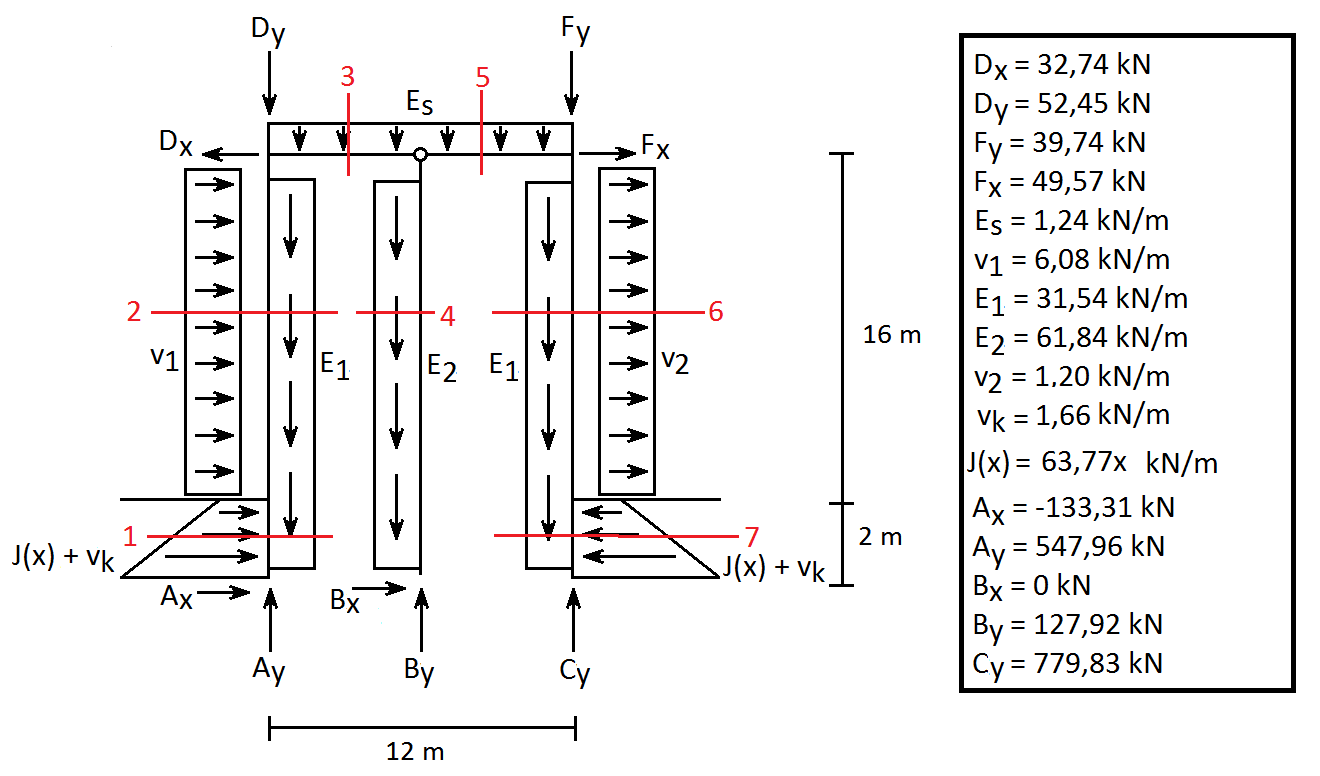
\includegraphics[width=0.8\textwidth]{billeder/snitbrud.png}
	\caption{Snit}
	\label{fig:snitbrud}
\end{figure}

Nedenfor vises beregningseksempel for snit 1 og snit 5. Beregningerne for de resterende snit kan ses i Bilag ???. 
\newline
\newline
\textbf{Snit 1: 0 m < x < 2 m}
\newline
Fritlegemediagrammet for snit 1 ses på Figur \ref{fig:snitet}.
\newline
\newline
Først bestemmes normalkraften:
\begin{center}
	$0 = N_1 + A_y - E_1 \cdot x \leftrightarrow N_1(x) = 31,\!54 \frac{kN}{m} x - 547,\!95 kN $
\end{center}

Normalkraften bestemmes ved 0 m og 2 m:
\begin{center}
	$N_1(0m) = -547,\!95 kN$ og	$N_1(2m) = -484,\!87 kN$
\end{center}

Nu bestemmes forskydningskraften:
\begin{center}
	$0 = V_1 + J(x) + v_k \cdot x + A_x \leftrightarrow V_1(x) = -33,\!64\frac{kN}{m} x + 133,\!31 kN$
\end{center}

Forskydningskraften bestemmes ved 0 m og 2 m:
\begin{center}
	$V_1(0m) = 133,\!31 kN$ og $V_1(2m) = 66,\!02 kN$
\end{center}

Til sidst bestemmes momentkraften:
\begin{center}
	$0 = M_1 + J(x) \cdot \frac{2x}{3} + v_k \cdot x \cdot \frac{x}{2} + A_x \cdot x \leftrightarrow M_1(x) = -22,\!15\frac{kN}{m} x^2 + 133,\!30kN x$
\end{center}

Momentkraften i højden 0 m og 2 m bestemmes:
\begin{center}
	$M_1(0m) = 0 kNm$  og $M_1(2m) = 178,\!00 kNm$
\end{center}

\begin{figure}[H]\centering
	\begin{minipage}[b]{0.48\textwidth}\centering
		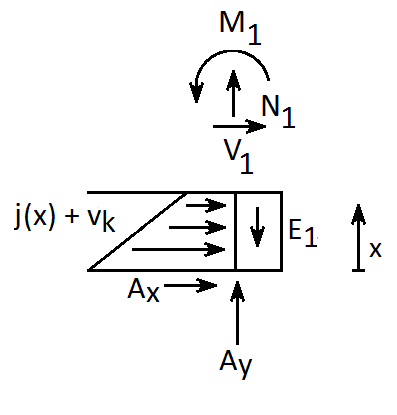
\includegraphics[width=0.80\textwidth]{billeder/snitet.png} %Venstre billede
	\end{minipage}\hfill
	\begin{minipage}[b]{0.48\textwidth}\centering
		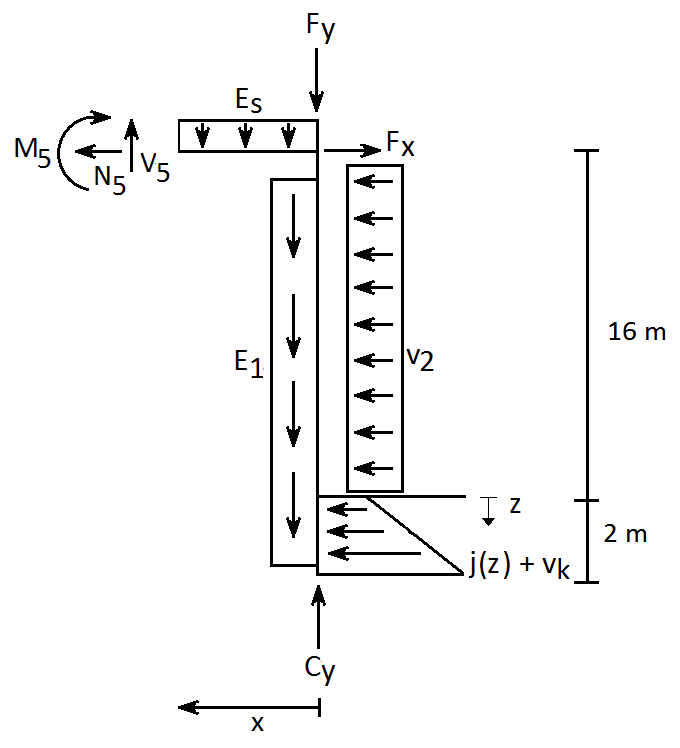
\includegraphics[width=1.0\textwidth]{billeder/snitfem.png} %Højre billede
	\end{minipage}\\ %Captions and labels
	\begin{minipage}[t]{0.48\textwidth}
		\caption{Fritlegemediagram for snit 1} %Venstre caption og label
		\label{fig:snitet}
	\end{minipage}\hfill
	\begin{minipage}[t]{0.48\textwidth}
		\caption{Fritlegemediagram for snit 5} %Højre caption og label
		\label{fig:snitfem}
	\end{minipage}
\end{figure}

\textbf{Snit 5: 0 m < x < 6 m}
\newline
Fritlegemediagrammet for snit 1 ses på Figur \ref{fig:snitfem}.
\newline
\newline
Normalkraften bestemmes først:
\begin{center}
	$0 = -N_5 + F_x - v_2 \cdot 16m - J(2m) - v_k \cdot 2m \leftrightarrow N_5 = 49,\!57 kN - 48,\!12 kN = 1,\!45 kN$
\end{center}

Hermed er normalkraften til 0 m og 6 m 1,45 kN. 
\newline
\newline
Forskydningskraften for snit 5 bestemmes ved:
\begin{center}
	$0 = V_5 - E_1 \cdot 18 m - F_y + C_y - E_s x \leftrightarrow V_5(x) = -172,\!35 kN + 1,\!24 \frac{kN}{m}x$
\end{center}

Forskydningskraften til 0 m og 6 m er hermed:
\begin{center}
	$V_5(0m) = -172,\!35 kN$ og $V_5(6m) = -164,\!89 kN$
\end{center}

Til sidst bestemmes momentkraften:
\begin{center}
	$0 = -M_5 - F_y \cdot x - E_1 \cdot 18 m \cdot x - E_s \cdot x \frac{x}{2} - v_2 \cdot 16 m \cdot 8 m - v_k \cdot 2 m \cdot 17 m - J(2m) \cdot 17,\!33 m + C_y \cdot x \leftrightarrow M_5(x) = 172,\!35 kN \cdot x - 0,\!62 \frac{kN}{m} \cdot x^2 -1011,\!72 kNm$
\end{center}

Momentkraften til 0 m og 6 m bestemmes:
\begin{center}
	$M_5(0m) = -1011,\!72 kNm$ og $M_5(6m) = 0 kN$
\end{center}

Tabel \ref{tab:resultaterbrud} viser resultaterne for alle snittene, som bruges til at beregne spændingstilstanden. 

\begin{table}
	\begin{center}
		\begin{tabular}{|c|c|c|c|c|c|c|}
			\hline
			Snit/Værdi & N($x_{min}$) & N($x_{max}$) & V($x_{min}$) & V($x_{max}$) & M($x_{min}$) & M($x_{max}$) 	\\ \hline
			1, 0<x<2  & -547,95       & -484,87    	&  133,31    	&  66,02 	&  0,00     &  178.00        		\\ \hline
			2, 2<x<18 &  -484,87        &  19,78       &  53,85      & -43,46   &  178,00  &  455,80    \\ \hline
			3, 0<x<6  & 1,45       &  1,45     &  -72,24         &  -79,69     &  403,78     &  0,21 			    \\ \hline
			4, 0<x<18 &  -1027,92       &  85,20      &  0,00        &  0,00    &  0,00   &   0,00    \\ \hline
			5, 0<x<6  &  1,45     &    1,45      &  -172,35      &  -164,89     &   -1011,72        &   0,00      		\\ \hline
			6, 2<x<18 &  -716,74  &   -212,09  &   -64,89    &   -45,73    &    -88,62       &   -1011,94      		\\ \hline
			7, 0<x<2 &  -779,83        &   -716,75       &     0,00      &   -67,29   &    0,00     &    -88,62     		\\ \hline
		\end{tabular}
		\caption{Snitkræfter for brudgrænsetilstand, N og V: kN og M: $kNm$}
		\label{tab:resultaterbrud}
	\end{center}
\end{table}

Ud fra snittene er der lavet snitkurver, som er illusteret på Figur \ref{fig:forskydningskurve}, Figur \ref{fig:momentkurve} og Figur \ref{fig:normalkraftkurve}. Værdierne i kurverne aflæses i Tabel \ref{tab:resultaterbrud}, hvor $V_1$ angiver værdien for forskydningskraften ved snit 1. Altså er $V_1(0m) = 133,31 kN$, $V_1(2m) = 66,02 kN$, osv.

\begin{figure}[H]
	\centering
	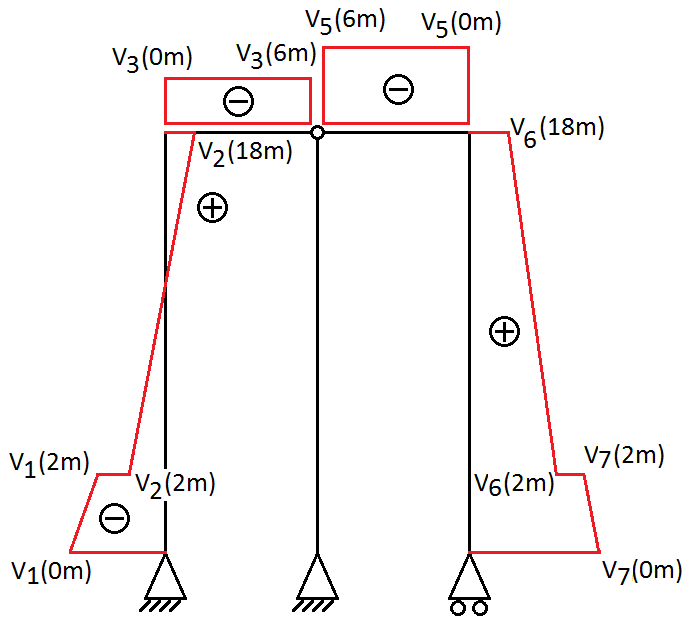
\includegraphics[width=0.7\textwidth]{billeder/sk.png}
	\caption{Forskydningskurve}
	\label{fig:forskydningskurve}
\end{figure}

\begin{figure}[H]
	\centering
	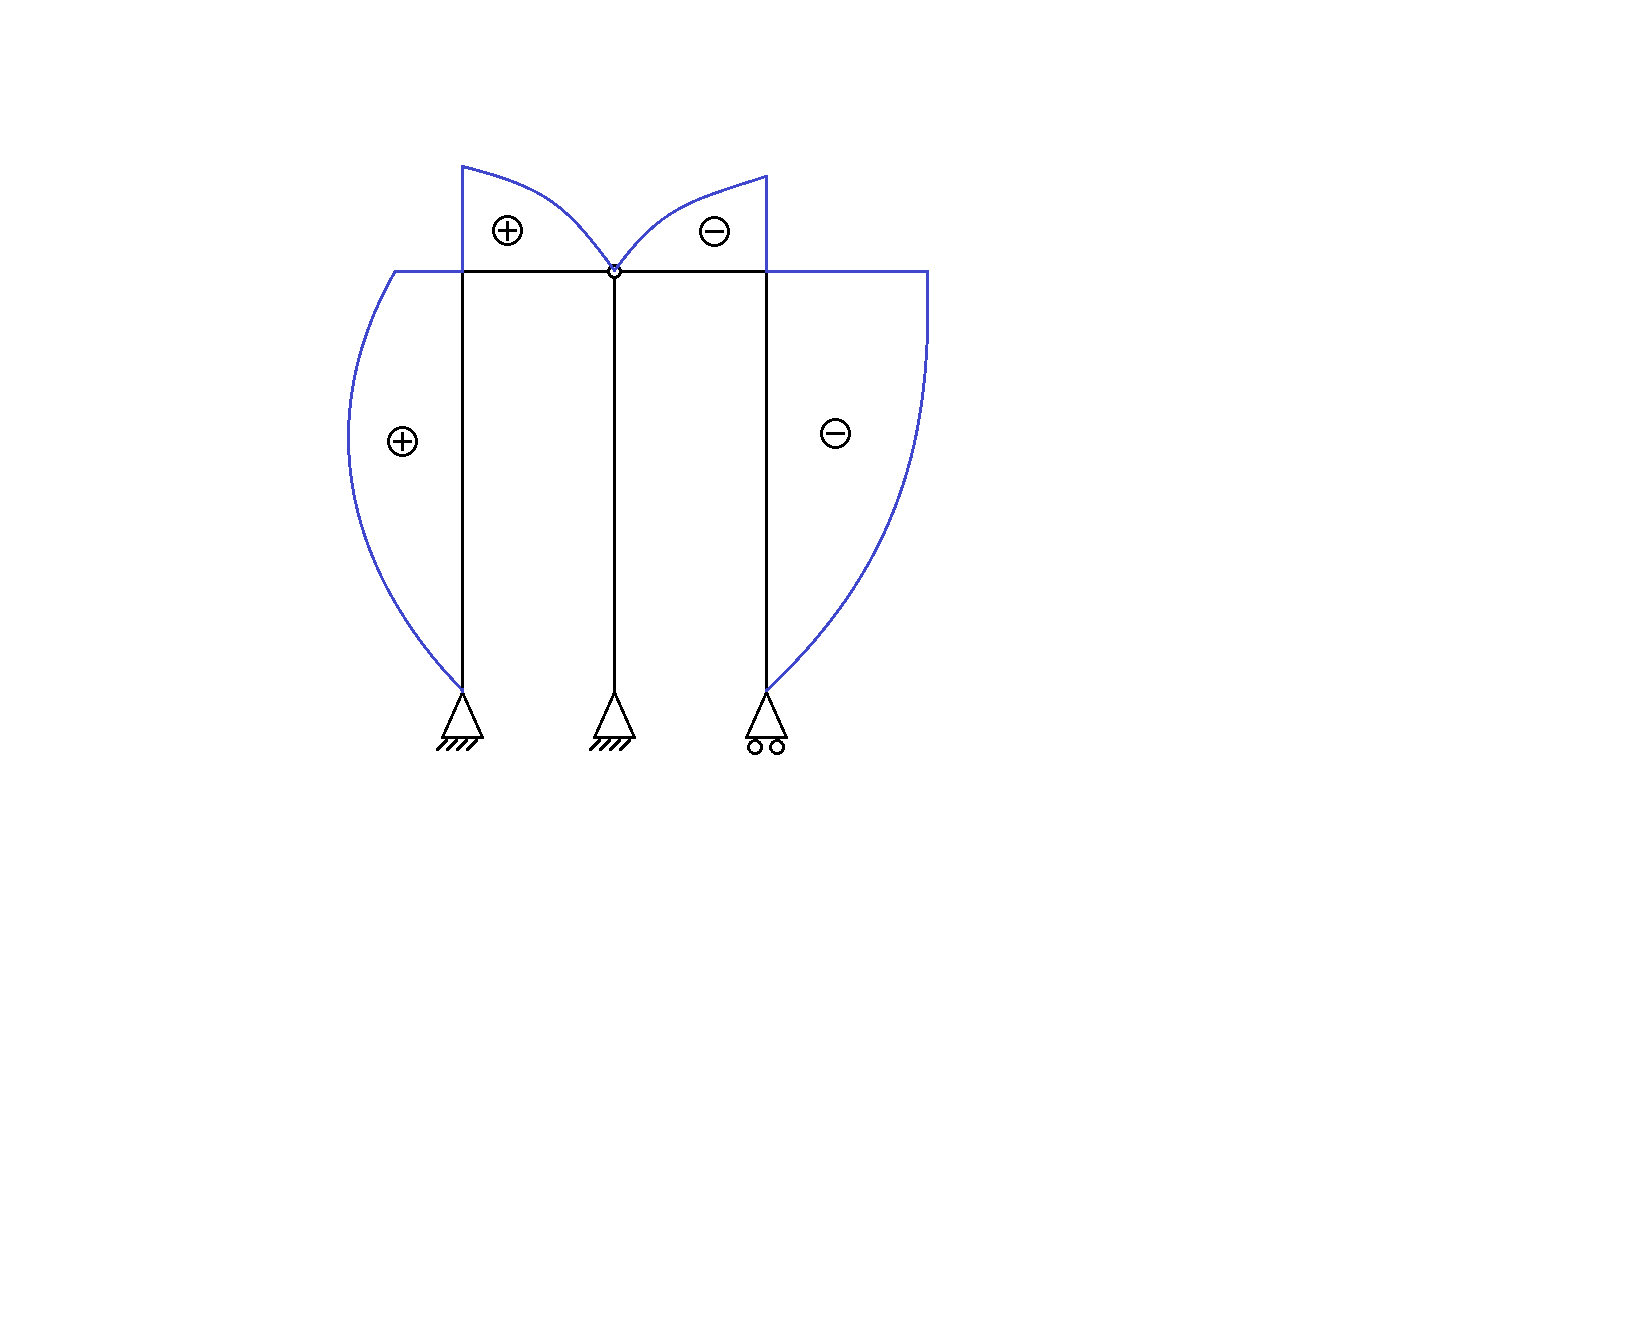
\includegraphics[width=0.7\textwidth]{billeder/skkm.png}
	\caption{Momentkurve}
	\label{fig:momentkurve}
\end{figure}

\begin{figure}[H]
	\centering
	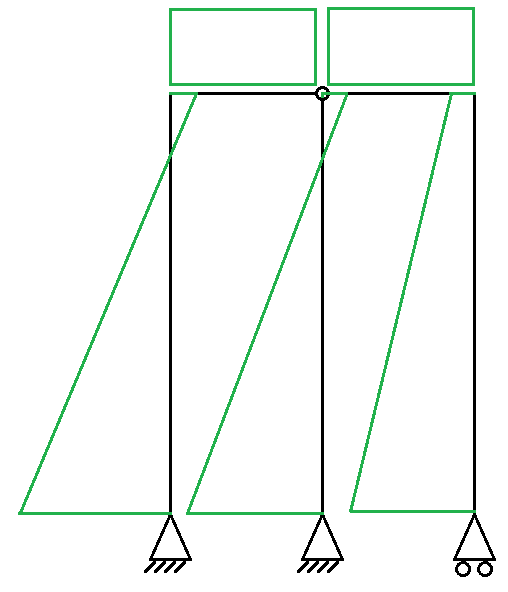
\includegraphics[width=0.7\textwidth]{billeder/SKFN.png}
	\caption{Normalkraftkurve}
	\label{fig:normalkraftkurve}
\end{figure}

\section{Spænding}
\begin{figure}[H]
	\centering
	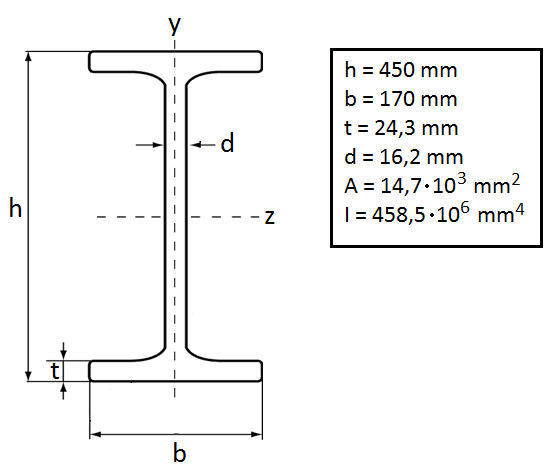
\includegraphics[width=0.4\textwidth]{billeder/iprofil.png}
	\caption{I-profil 450}
	\label{fig:iprofil}
\end{figure}

For at finde ud af om konstruktionen kan holde, undersøges spændingstilstanden. Her skal det gælde:

\begin{center}
	$\sqrt{\sigma^2 + 3\tau^2} \le f_y$ 
\end{center}

\begin{itemize}
	\item[-] $\sigma$: Normalspænding [MPa]
	\item[-] $\tau$: Forskydningsspænding [MPa]
	\item[-] $f_y$: Flydespænding [MPa]
\end{itemize}

Flydespændingen beregnes ved formlen:

\begin{center}
	$f_y = \frac{f_{yk}}{\gamma}$
\end{center}

\begin{itemize}
	\item[-] $f_{yk}$: Den karakteristiske flydespænding, der afhænger af ståltype. For ståltype S235 er $f_{yk} = 225 MPa$
	\item[-] $\gamma$: Partialkoefficient, der sættes til 1,1 \citep[ s. 212]{stabi}.  
\end{itemize}

Altså beregnes den regningsmæssige flydespænding til:

\begin{center}
	$f_y = \frac{225 MPa}{1,\!1} = 204,\!54 MPa$
\end{center}

Normalspændingen findes ved Naviers formel:

\begin{center}
	$\sigma = \frac{N}{A} - \frac{M}{I} y$
\end{center}

\begin{itemize}
	\item[-] N: Normalkraft [kN], som er bestemt igennem snitkræfter
	\item[-] A: Tværsnitsareal, som for stålprofil 450 er $14,\!7 \cdot 10^3 mm^2$ \citep{stabi}. 
	\item[-] M: Moment [kN], som er bestemt igennem snitkræfter
	\item[-] y: Tyngdepunktskoordinat [mm], som er $\pm 225$
	\item[-] I: Inertimoment, som for stålprofil 450 er $458,\!5 \cdot 10^6 mm^4$ \citep{stabi}. 
\end{itemize} 

Dernæst beregnes forskydningsspændingen ved Grasshofs formel:

\begin{center}
	$\tau = \frac{VQ}{Ib}$
\end{center}

\begin{itemize}
	\item[-] V: Forskydningskraft [kN], som er bestemt igennem snitkræfter
	\item[-] Q: 1. ordens arealmoment for $A_1$: $Q = \int_{A_1}y \mathrm{d}A = yA$ $[mm^3]$
	\item[-] b: bredde, som er 24,3 mm
\end{itemize}

Nedenfor vises et beregningseksempel for et kritisk punkt. Resultaterne for alle de valgte kritiske punkter kan ses på Figur \ref{fig:tabelspanding}. 
\newline
\newline
\textbf{Snit 5: Største forskydningskraft}
\newline
Normalspændingen og forskydningsspændingen beregnes begge ved henholdsvis $y = -225 mm$ og $y = 225 mm$, fordi I-profilens højde er 450 mm, og dermed er længden til y-koordinaten $\pm 225 mm$. Eksemplet nedenfor, er beregnet med $y = 225 mm$.

Først beregnes normalspændingen:
\begin{center}
	$\sigma = \frac{1,\!45 kN}{14,\!7 \cdot 10^3 mm^2} - \frac{-1011,\!72 kNm}{458,\!5 \cdot 10^6 mm^4} \cdot 225 mm = 496,\!58 MPa$
\end{center}

Dernæst beregnes forskydningsspændingen:
\begin{center}
	$\tau = \frac{-172,\!35 kN \cdot (225 mm \cdot 14,\!7\cdot10^3 mm^2)}{458,\!5\cdot10^6 mm^4 \cdot 24,\!3 mm} = -51,\!16 MPa$
\end{center}

Til sidst kan spændingstilstanden beregnes:
\begin{center}
	$\sqrt{496,\!58^2 MPa + 3 \cdot (-51,\!16)^2 MPa} = 504,\!43 MPa$
\end{center}

Denne spænding på 504,43 MPa, er for høj, idet flydespændingen er beregnet til $204,\!54 MPa$. Dermed vil konstruktionen bryde sammen.

 \begin{figure}[H]
 	\centering
 	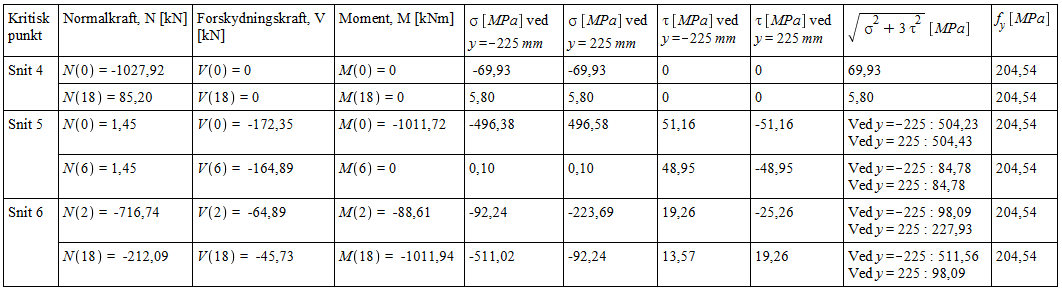
\includegraphics[width=1.1\textwidth]{billeder/tabelspanding.png}
 	\caption{Resultater af spændingstilstand}
 	\label{fig:tabelspanding}
 \end{figure}

Det ses på Figur \ref{fig:tabelspanding}, at spændingen i flere tilfælde overskrider den regningsmsæssige flydespænding. Derfor vil stålrammen opleve brud og i værste tilfælde knække sammen, som det kendes fra ståls arbejdskurve.
\newline 
\newline
For at konstruktionen ikke skal bryde sammen, skal der foretages en række ændringer.
\newline \indent{     }  Der er indsat tre stålrammer i tilbygningen. Ved at indsætte en eller to stålrammer mere, vil lasterne fordeles ud over disse, og dermed vil hver enkelt stålramme belastes mindre. Dermed vil spændingerne i sidste ende mindskes. 
\newline \indent{     }  Der er valgt en ståltype S235, som kan ændres til en højere styrkeklasse, for eksempel S275 eller S355. Ved at vælge en højere styrkeklasse, øges flydespændingen dermed. En større flydespænding betyder, at stålen kan klare en større spænding. Ved for eksempel kan ændre ståltypen til S355 ændres flydespændingen til $f_y = \frac{345 MPa}{1,\!1} = 313,\!64 MPa$. Dette er dog stadig ikke en stærk nok stål, og derfor kan dette ikke være den eneste ændring der skal foretages. 
\newline \indent{     }  Til sidst kan der vælges en anden stålprofil. Dette vil ændre henholdsvis højde, bredde, inertimomentet, densiteten, tværsnitsarealet, m.m. på stålprofilen. Dette vil give anledning til en mindre egenlast, hvis stålprofilen mindskes, og dermed en mindre spænding.
\newline
\newline
Helt så simpelt kan det dog ikke opstilles, da der for et rigtigt byggeprojekt også skal tages højde for det økonomiske aspekt af byggeriet, og omkostningerne. Hvis ikke leverandøren har en stærkere ståltype end S235 på lager, så kan omkostningerne hurtigt løbe op, når man er på udkig efter en stærkere type som eksempelvis S355, og det er derfor ikke muligt bare at vælge ståltype efter ønske, da det er omkostningsfuldt.